%%%%%%%%%%%%%%%%%%%%%%%%%%%%%%%%%%%%%%%%%
% Minimalist Book Title Page 
% LaTeX Template
% Version 1.0 (27/12/12)
%
% This template has been downloaded from:
% http://www.LaTeXTemplates.com
%
% Original author:
% Peter Wilson (herries.press@earthlink.net)
%
% License:
% CC BY-NC-SA 3.0 (http://creativecommons.org/licenses/by-nc-sa/3.0/)
% 
% Instructions for using this template:
% This title page compiles as is. If you wish to include this title page in 
% another document, you will need to copy everything before 
% \begin{document} into the preamble of your document. The title page is
% then included using \titleTH within your document.
%
%%%%%%%%%%%%%%%%%%%%%%%%%%%%%%%%%%%%%%%%%

%----------------------------------------------------------------------------------------
%	PACKAGES AND OTHER DOCUMENT CONFIGURATIONS
%----------------------------------------------------------------------------------------

%\title{Embedded Sytem Design: The GOAT}

\documentclass[10pt,a4paper]{article}

\usepackage[utf8]{inputenc}
\usepackage[T1]{fontenc}
\usepackage[svgnames]{xcolor} % Required to specify font color
\usepackage{mathpazo}
\usepackage{floatrow}
\usepackage{geometry}%réglages mise en page
\geometry{%
a4paper, % note : l'option a4paper tuait la marge supérieure.
body={170mm,250mm}, %
left=25mm,top=25mm,right=25mm, %
headheight=21mm,headsep=7mm,
marginparsep=4mm,
marginparwidth=20mm, %
footnotesep=50mm
}

\usepackage{graphicx}
\usepackage{float}
\usepackage{color}
\usepackage{amssymb}

%\usepackage[boxed]{algorithm2e}
\usepackage{array}
\usepackage{hyperref}
\usepackage{lscape}

%%% Pour colorier le code source C++/matlab
\usepackage{listings}
\usepackage{xcolor}
\usepackage[colorinlistoftodos]{todonotes}

\newcommand*{\course}{\fbox{INFO-F-410}} % Generic publisher logo


%----------------------------------------------------------------------------------------
%	TITLE PAGE
%----------------------------------------------------------------------------------------

\newcommand*{\titleTH}{\begingroup % Create the command for including the title page in the document
\raggedleft % Right-align all text
\vspace*{\baselineskip} % Whitespace at the top of the page

{\Large \textsc{Anthony Debruyn}}\\[0.01\textheight] % Author name
{\Large \textsc{Brian Delhaisse}}\\[0.01\textheight] % Author name
{\Large \textsc{Quentin Delhaye}}\\[0.167\textheight] % Author name

{\LARGE\bfseries Embedded Systems Design}\\[\baselineskip] % First part of the title, if it is unimportant consider making the font size smaller to accentuate the main title

{\textcolor{green}{\Huge The GOAT}}\\[\baselineskip] % Main title which draws the focus of the reader

{\Large \textit{The Gate Opener Actioned by Ticket}}\par % Tagline or further description

\vfill % Whitespace between the title block and the publisher

%\vspace*{30\baselineskip} % Whitespace at the bottom of the page

{\large \textsc{Gilles Geraerts} \course}\par % Publisher and logo

%\vspace*{5\baselineskip} % Whitespace at the bottom of the page
\endgroup}

%----------------------------------------------------------------------------------------
%	BLANK DOCUMENT
%----------------------------------------------------------------------------------------

%%%%%%%%%%%%%%%%%%%%%%%%%%%%%%%%%%%%%%%%%%%%%%%%%%%%%%%%%%%%%%%%%%%%%%%%
%%
%%    Environnement coloré pour écrire des codes.
%%
%%      Environnement :
%%       lstlisting
%%
%%      UTILISATION :
%%
%%         \lstset{language=c++}
%%         \lstset{commentstyle=\color{colComments}\textit}
%%         \begin{lstlisting}
%%             CODE
%%         \end{lstlisting}
%%
%%
%%%%%%%%%%%%%%%%%%%%%%%%%%%%%%%%%%%%%%%%%%%%%%%%%%%%%%%%%%%%%%%%%%%%%%%%

\definecolor{colKeys}{rgb}{0,0,1}  % couleurs des mots-clés propres au language
\definecolor{colIdentifier}{rgb}{0,0,0}  % couleurs des mots à identifier
\definecolor{colComments}{rgb}{0,0.6,0}  % couleurs des commentaires
\definecolor{colString}{rgb}{0.6,0.1,0.1}
%\lstset{}

%%%%%%%%%%%%%%%%%%%%%%%%%%%%%%%%%%%%%%%%%%%%%%%%%%%%%%%%%%%%%%%%%%%%%%%%%%%%%%%%%%%

\begin{document} 

\thispagestyle{empty}

\titleTH % This command includes the title page

\newpage

\tableofcontents
\newpage
%%%%%%%% Introduction %%%%%%%%%%
\section{Introduction}
For the course "Embedded Systems Design", we were asked to implement a system inspired from subject in the course. We chose to use UppAal Tiga to design and create a strategy for a sas controlled by an Arduino Uno. This sas is composed of 2 doors actioned by servomotors. Infrared sensors are used to detect the person entering the sas. The opening of the second door of the sas is triggered by the scan of a valid card (rectangle with holes). Once someone is inside the sas, a timer is triggered to prevent the person to stay indefinitely inside. An alarm is activated once the timer is out.

%%%%%%%% The Model %%%%%%%%%%%%
\section{The Model}

In this section we will describe the physical properties that the system must satisfy, and make the link with the model.\\

First we want the system to always have at least one door closed. This is ensured by the 3 available configurations in the model: \emph{01} meaning door 1 open and door 2 closed, \emph{10} meaning the opposite, and \emph{00} meaning no door open.\\

Secondly, we want the back door (door 2) to open only if the user present one valid card having 2 holes in it.\\

The user also has to be ejected after some time if he does not show a valid card. This would prevent the user from staying indefinitely in the sas, blocking the other users. This is done by the timer in the model for the sas and the eject message. \\

The sas must detect the insertion of a card, even if it is not valid. This is modeled with the cardIn message in the UppAal Tiga systems.\\

An infrared sensor system has to detect the entry and exit of the user in order to react with the appropriate door configuration, and (de)activate the alarm. In the model, the infrared sensors are modeled with the infra1 \& infra2 signal.

The user must be able to escape the sas at any time. This is done with the infra1 sensor. If the user puts himself in front of the sensor, the front door opens to let him out.

The figures~\ref{userModel} and \ref{sasModel} represent these and the listings~\ref{globalDecl}, \ref{userDecl} and \ref{sasDecl} are their declarations.

A Typical run on the user side is as follows: The user begins in \texttt{before\_sas} and proceed into the sas by triggering the \texttt{infra1} signal if the first door is opened. He enters either with a valid or invalid card.
Once in the sas, he can present his card by triggering the \texttt{cardIn} signal.
At any moment, if the second door is opened, he can leave through it, or leave through the first door by triggering the signal \texttt{infra1}.
If the global clock \texttt{timeInSas} exceeds \texttt{SAS\_TIMER}, he can go to the \texttt{FAIL} state, and when receiving the \texttt{eject} signal, he will leave the sas.

A typical run on the sas side is as follows: From the \texttt{idle} state, uppon \texttt{infra1} signal, the sas resets the clock \texttt{timeInSas} and closes the first door. 
The sas is then handling a user. 
When a detects that a card is entered, he either opens the second door if the card is correct but keep both closed if the card is invalid.
If he receives the signal \texttt{infra1}, it means that user is standing in front of the first sensor and wants to leave, hence the sas opens the first door.
Whenever the \texttt{timeInSas} clock reaches the \texttt{SAS\_TIMER}, the sas immediatly triggers the \texttt{eject} signal, willing to make the user leave the bloody sas.


\begin{figure}[!h]
	\centering
    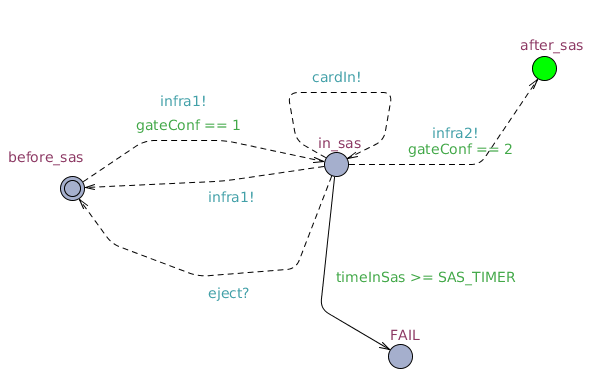
\includegraphics[width=\textwidth]{User_model.png}
    \caption{The user model}
    \label{userModel}
\end{figure}

\begin{figure}[!h]
	\centering
    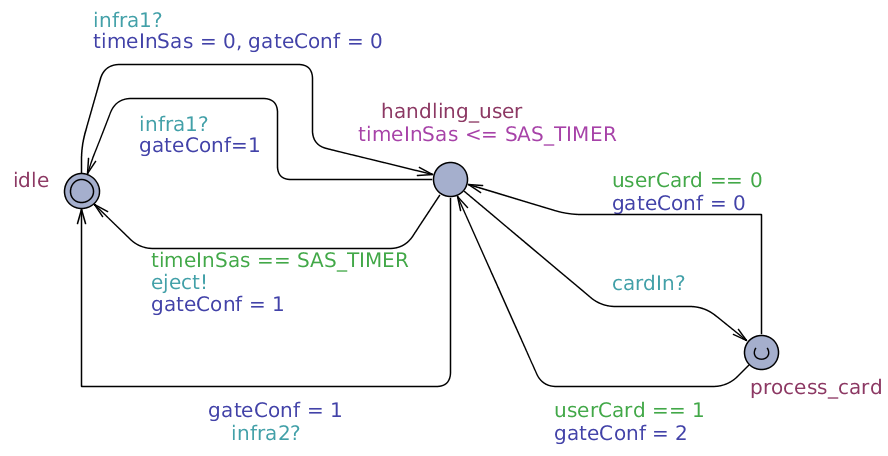
\includegraphics[width=\textwidth]{sasModel.png}
    \caption{The sas model}
    \label{sasModel}
\end{figure}

\lstset{language=c++}
\lstset{commentstyle=\color{colComments}\textit,
%float=hbp,%
basicstyle=\ttfamily\small, %
identifierstyle=\color{colIdentifier}, %
keywordstyle=\color{colKeys}, %
stringstyle=\color{colString}, %
commentstyle=\color{colComments}, %
columns=flexible, %
tabsize=2, %
%frame=trBL, %
%frameround=tttt, %
extendedchars=true, %
showspaces=false, %
showstringspaces=false, %
numbers=left, %
numberstyle=\tiny, %
breaklines=true, %
breakautoindent=true, %
captionpos=b,%
%xrightmargin=-0.6cm, %
%xleftmargin=-0.6cm}
}
\begin{lstlisting}[caption=Global declarations of the systems., label=globalDecl]
chan infra1, infra2, cardIn, eject;
clock timeInSas;
const int SAS_TIMER = 10;
int gateConf = 1;
int userCard;
\end{lstlisting}
\begin{lstlisting}[caption=Declarations of the user model., label=userDecl]
clock x;
\end{lstlisting}
\begin{lstlisting}[caption=Declarations of the sas model., label=sasDecl]
clock x;
\end{lstlisting}

%%%%%%%%%%%%%%%%%%%%%%%%%%%%%%%%%
\section{The Strategy}
%%%%%%%%%%%%%%%%%%%%%%%%%%%%%%%%%
\subsection{Winning conditions}

\begin{description}
	%\item[\texttt{A<> not(User.FAIL)}] ~\\
    %	The user will never end up in FAIL.
        
    \item[\texttt{A[] not(User.in\_sas and User2.in\_sas)}] ~\\     
    Both users are never in the sas at the same time.
    Both models are exactly the same. The managment of a request token and a users queue will be implemented for the Formal Verification project.
    
    %\item[\texttt{A[] not deadlock}] ~\\
    
    \item[\texttt{E<> User.after\_sas}] ~\\
    	It is possible for the user to reach the other side of the sas. He won't succeed on every try, but if he wants to, he will.

    \item[\texttt{A[] not (User.FAIL)}] ~\\
    	We want to verify if the user will always avoid the FAIL state.
        At the instant \texttt{timeInSas} = \texttt{SAS\_TIMER} the system has two choice: either take \texttt{Sas.handling\_user} to \texttt{Sas.idle}, or \texttt{User.in\_sas} to \texttt{User.before\_sas}.
        The FAIL state is thus reachable and the test is expected to fail.
    
    \item[\texttt{control: A[] not(User.FAIL or User2.FAIL)}] ~\\
    Here, we play in a controller game.
    Having the controller collaboration, when the system is given the opportunity to either win or lose, well, it chooses to win.
    This condition is there to enforce the limited time in sas property.
    
    Please bear in mind here that we suppose that the \texttt{eject!} signal sent by the \texttt{Sas} has force of law.
    Hence, we know that when the controller is trying to comply with a winning condition, our physical system will be able to overcome the quite strong hypothesis made by the simulation tool stating that the environnement is always able to act faster than the controller.
    This liberty is represented by the controllable edge between \texttt{User.in\_sas} and \texttt{user.FAIL}.
\end{description}

We may also want to verify that if the user enters the sas with an invalid card, he will not make it to the other side, but if he has a valid card, he may.
This may be expressed as follows:
\begin{small}
\begin{verbatim}
	A[] ( ( (userCard == 0 && User.in_sas) imply A<> User.before_sas ) 
	&& ( (userCard == 1 && User.in_sas) imply E<> User.after_sas ) )
\end{verbatim}
\end{small}

Sadly, the syntax analyzer of UppAal does not accept a quantifier after the keyword \texttt{imply} and the above condition is not verifiable through its tools.\\

Finally, one could think that a suitable strategy for the sas to avoid the user to enter the \texttt{FAIL} state would simply be to never open the first door and let users in.
However, the model construction is such that the first door is always open when the sas is not occupied.
The only way the close the first door is a user to enter the sas by triggering the \texttt{infra1} signal.

\subsection{Generated strategy}
The following strategy has been generated using a system with only one user for readability purposes.

\begin{verbatim}
Verifying property 5 at line 28
 -- Property is satisfied.
$v_gameInfoPlayInitial state:
( User.before_sas Sas.idle ) gateConf=1 
(timeInSas==User.x && User.x==Sas.x && Sas.x==0)

Strategy to avoid losing:

State: ( User.after_sas Sas.idle ) gateConf=1 
While you are in	true, wait.

State: ( User.before_sas Sas.idle ) gateConf=1 
While you are in	true, wait.

State: ( User.in_sas Sas.handling_user ) gateConf=2 
While you are in	(timeInSas<=10), wait.

State: ( User.in_sas Sas.process_card ) gateConf=0 
When you are in (timeInSas<=10), 
	take transition Sas.process_card->Sas.handling_user { 1, tau, gateConf := 2 }

State: ( User.in_sas Sas.process_card ) gateConf=2 
When you are in (timeInSas<=10), 
	take transition Sas.process_card->Sas.handling_user { 1, tau, gateConf := 2 }

State: ( User.in_sas Sas.handling_user ) gateConf=0 
While you are in	(timeInSas<=10), wait.
\end{verbatim}

The implementation code is presented in appendix~\ref{ap:code}. Each of those states were implemented using \texttt{if-then-else} statements decorated with all kind of computation that were hidden behind abstractions in the models.

\section{Physical Implementation}
\subsection{Parts list}
For our prototype, we used:
\begin{itemize}
	\item a microcontroller: Arduino UNO.
	\item 5 resistances (220$\Omega$).
    \item 3 leds (1red, 1yellow, 1green).
    \item 2 analog servo motors (FS5103B).
    \item 2 infrared proximity sensors short range.
    \item 2 photoresistors.
    \item 1 micro switch (DM3).
    \item 1 buzzer.
    \item 1 battery pack holder for 4x AA batteries + the 4xAA batteries.
    \item jump wires.
    \item 3 half-size protoboards.
\end{itemize}

\subsection{Electronic schematic}

\begin{figure}[!h]
	\centering
    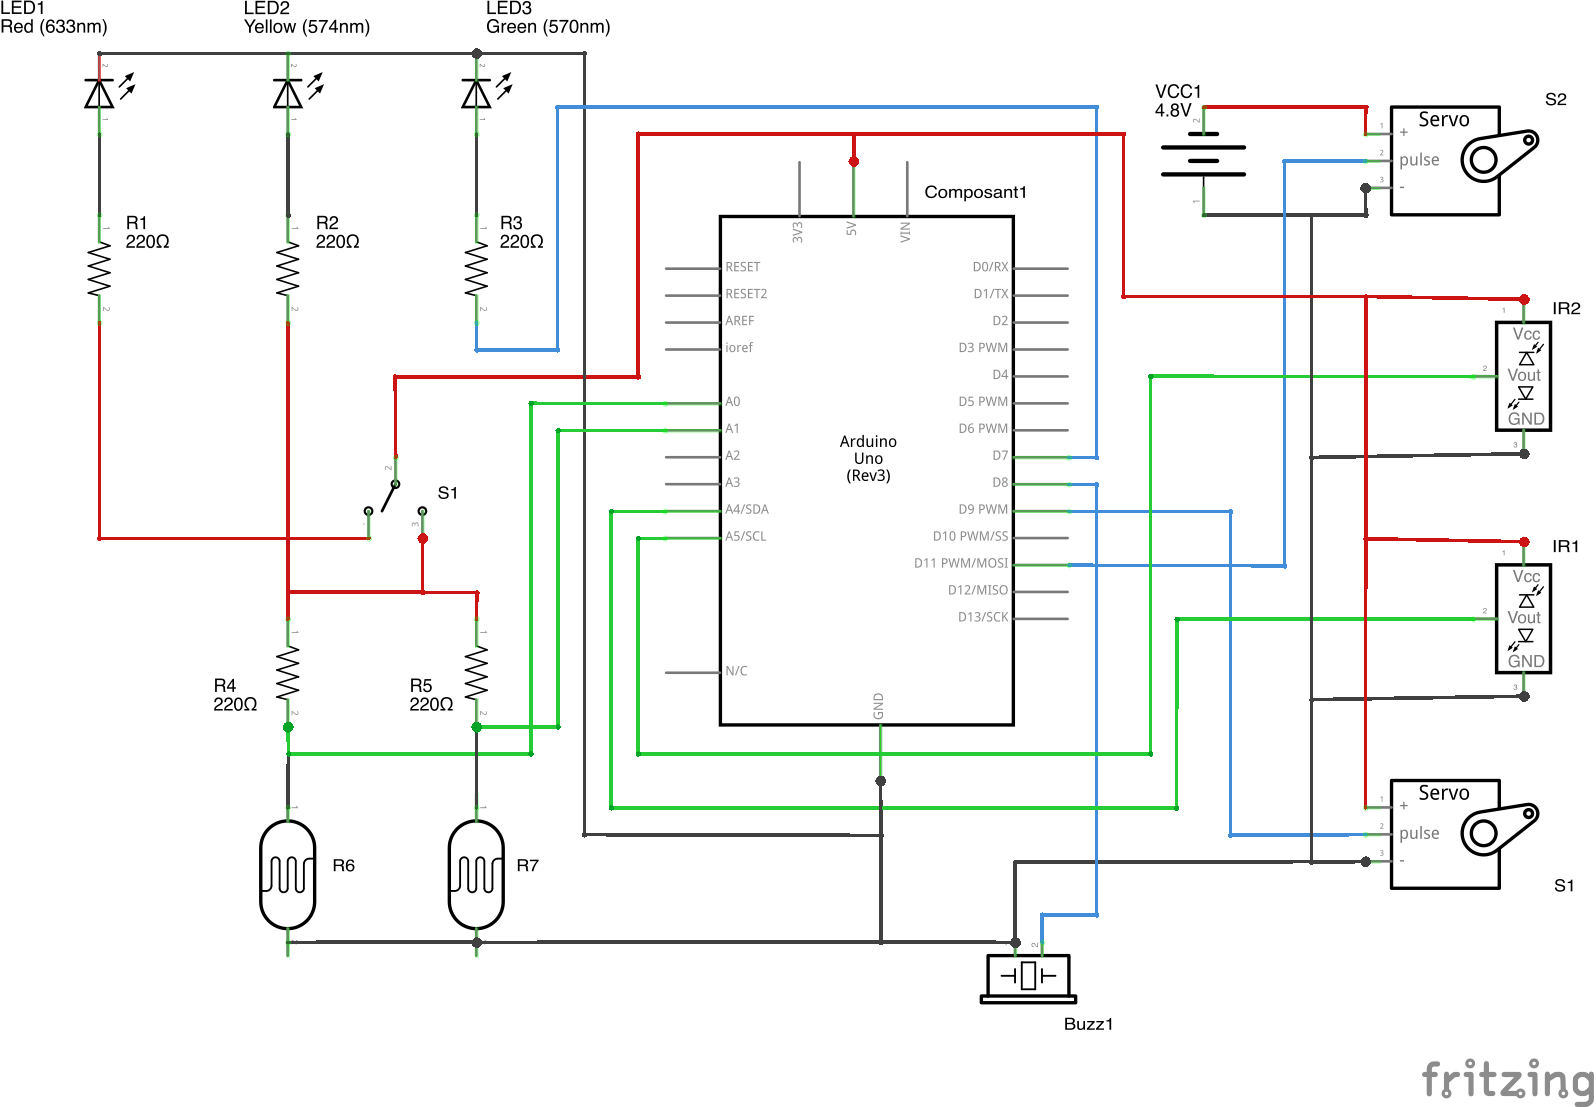
\includegraphics[scale=1]{ElectronicScheme1.png}
    \caption{Electrical diagram (modeled with Fritzing). Legend: \textcolor{red}{red wires} are connected to the positive terminal (of the arduino or the external battery), black wires are connected to the ground, \textcolor{green}{green wires} connect the electrical components to the analog input pins, and the \textcolor{blue}{blue wires} connect electrical components to digital output pins.}
    \label{elecScheme}
\end{figure}

Once the arduino is connected to a computer or to a battery, the positive terminal of the arduino supplies a tension of 5V to the electrical system, which can be seen on the figure \ref{elecScheme}. Because the servo motors drain a lot of current, another external battery was needed to supply enough current for both servo motors. Thus, an external battery has been connected to one of the servo. To avoid any other problems, we connected the ground of this one to the same ground as the arduino.

The resistors in front of each led are there so that the leds don't overdrive and burn out. The red led is always on until a card is inserted into the system. The card will push on the lever of the micro switch leading to the yellow led to turn on, and to the current to flow into the photoresistors.

The 2 resistors R4 and R5 with the photoresistors R6 and R7 form respectively a voltage divider. The voltage measured differs with the intensity of the light, that is, brighter the light is smaller the resistance of the photoresistor is. The resulting tension of those dividers are measured on the analog input pins A0 and A1 of the arduino. If the tension of each photoresistor is between a certain value, then the microcontroller is programmed to turn on the green led, and activate the 2nd servo motor (S2) in order to open the last door of the sas. 

If the user stays too long in the sas, the arduino can also trigger an alarm with the buzzer.

The 2 infrared proximity sensors IR1 and IR2 are there to detect if an object/person has entered or leaved the sas, they are respectively connected to the analog input pins A4 and A5. Based on the value measured, the microcontroller will activate one of the servo motors to close one of the gates, or to stop the buzzer.

\subsection{Electronic circuit}
On the real circuit, we used 3 breadboards because of the jump wires length that were too short. The 2 left protoboards on the figure \ref{circuit} are perpendicular to each other, in order to the card to be able to push on the lever of the micro switch, and to the photoresistors to be perpendicular to the card.

\begin{figure}[!h]
	\centering
    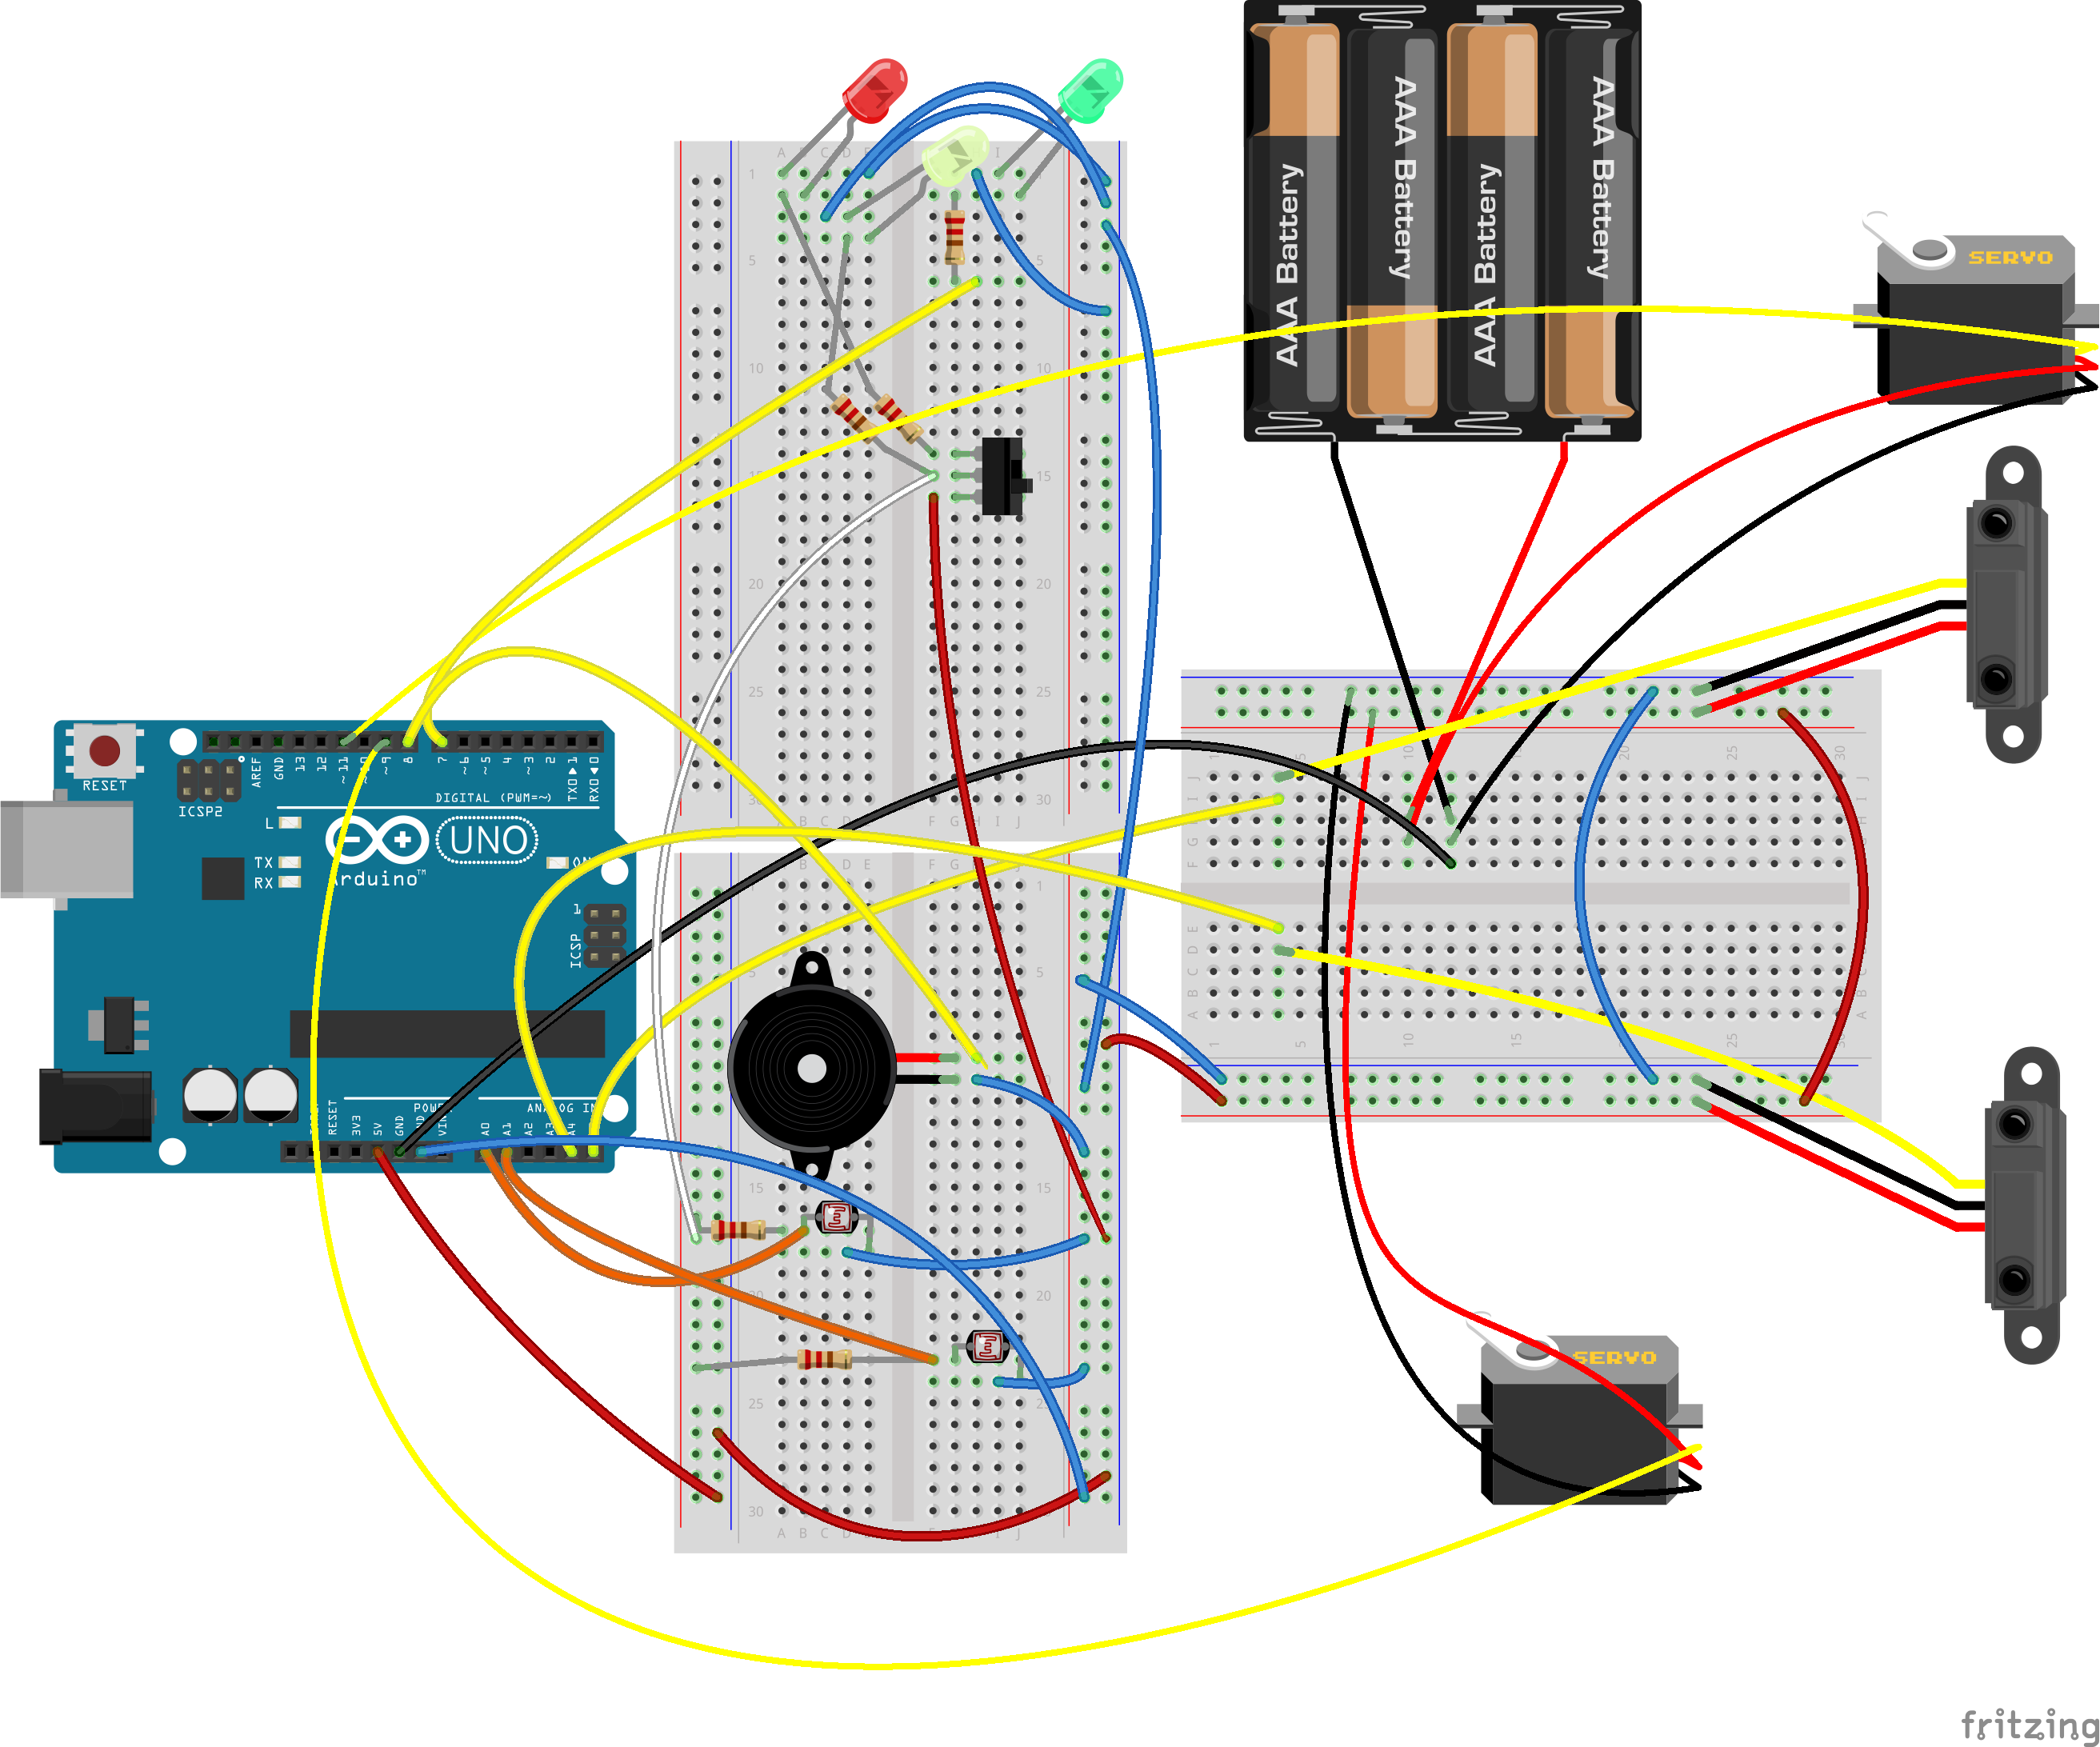
\includegraphics[scale=0.5]{ElectronicScheme2.png}
    \caption{The Circuit (modeled with Fritzing).}
    \label{circuit}
\end{figure}

\subsection{The structure}
The sas was build using Lego bricks, and the doors are in carton and connected to the servomotors with paperclips. We used cardboard to create some cards. A valid card has a hole in front of each photoresistor, so that the light can pass through it and be detected by the photoresistors. The final physical prototype can be found on the figure \ref{finalPrototype}.

%On figure \ref{inside}, the reader can view the inside of the sas. Here the first door is open, and the user is waiting.

%%%%%%%%%%%%%%%%%%%%%%
\section{Pictures of the project}
%%%%%%%%%%%%%%%%%%%%%
The final prototype can be seen on the following figure \ref{finalPrototype}.
\begin{figure}[!h]
	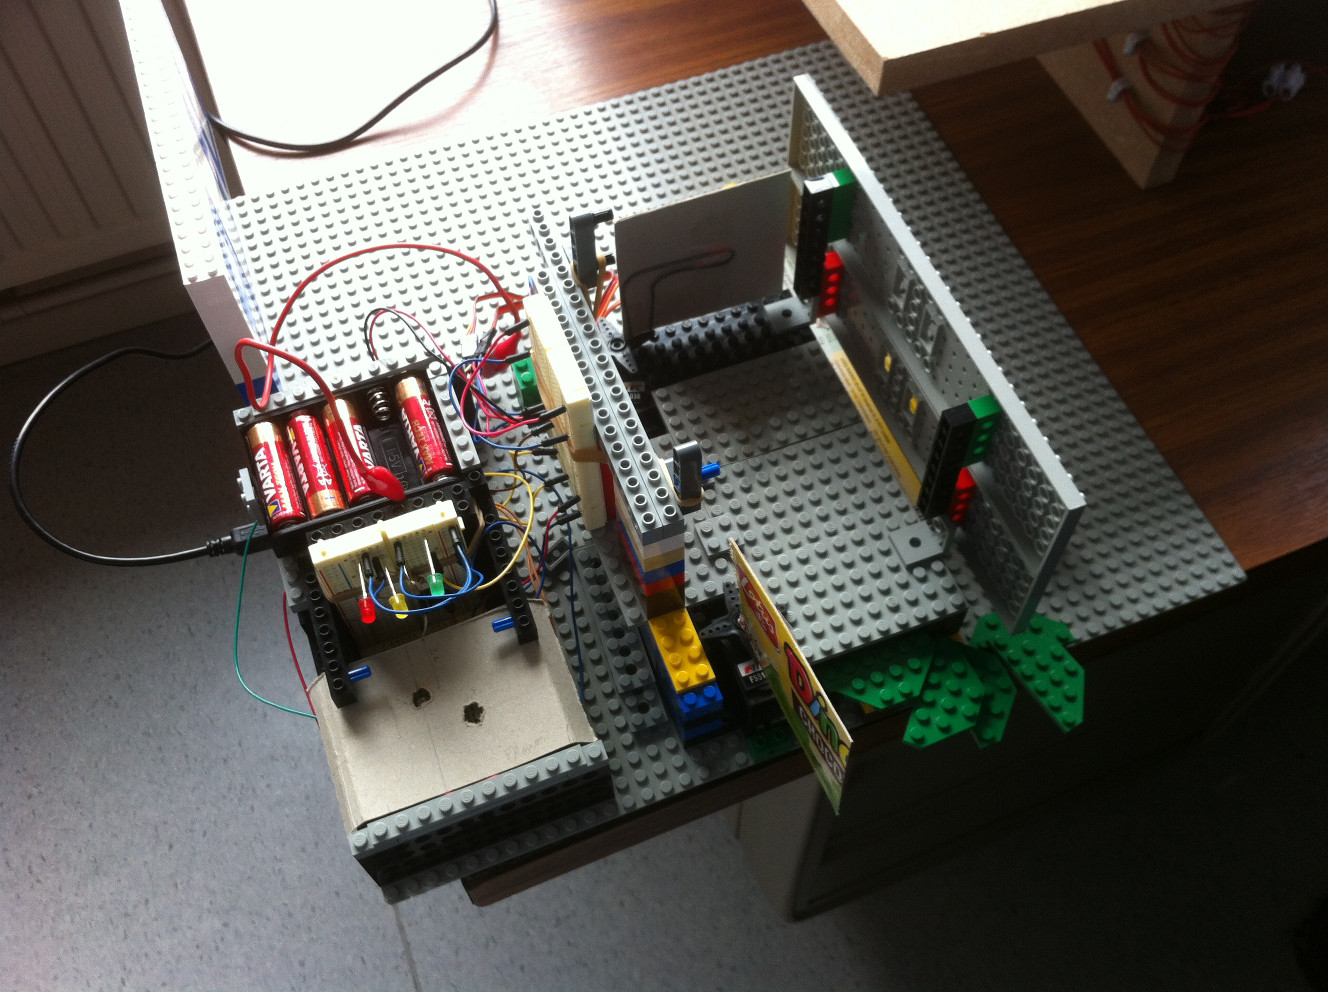
\includegraphics[scale=0.18]{photo1}
    \caption{Final prototype}
    \label{finalPrototype}
\end{figure}

\section{Future work}
Since we only use one infrared sensor at each door, we do not know the direction of the passing user. This causes problems in several situations:

\begin{itemize}
	\item If the user stays too long in the sas and the alarm activate, another user can enter in the sas. The alarm then stops. Now a third user can enter, and the front door closes. If one of the 2 users already in the sas puts something in front of the sensor, the front door closes as well. Thus any number of people enter the sas and go to the other side with one valid card.
    
    \item The same infrared problem occurs on the other side. If one user enters the sas from the back door when it is open, after the user has shown a valid card, the sas closes the second door. There are then 2 users in the sas, and the front door opens again, letting the second user escape.
	
\end{itemize}

These 2 problems could be resolved by using 2 more sensors to detect the direction of the passing user. Anoher solution could be to consider that the sas has only room for one person only.

%%%%%%%%%%%%%
\section{Conclusion}
%%%%%%%%%%%%%
This project has enabled us to understand how we design embedded systems, by using specific tools to verify that a system respect some given proprieties. It was a rich experience to do the different parts of a project: the design of the model, the production of the code from the generated strategies, and the physical implementation so that we can see that our model really works in the real world.


\newpage

\appendix

\section{Arduino Code}\label{ap:code}
As mentionned above, the following code has been produced based on the generated strategies.\\

\lstset{language=c++}
\lstset{commentstyle=\color{colComments}\textit,
float=hbp,%
basicstyle=\ttfamily\small, %
identifierstyle=\color{colIdentifier}, %
keywordstyle=\color{colKeys}, %
stringstyle=\color{colString}, %
columns=flexible, %
tabsize=2, %
frame=trBL, %
frameround=tttt, %
extendedchars=true, %
showspaces=false, %
showstringspaces=false, %
numbers=left, %
numberstyle=\tiny, %
breaklines=true, %
breakautoindent=true, %
captionpos=b,%
xrightmargin=-0.6cm, %
xleftmargin=-0.6cm}
\begin{lstlisting}
#include <Servo.h> 

Servo servo1;  // create servo object to control a servo 
Servo servo2; 

int pos1;    // variable to store the servo position 
int pos2;

const int ledPin = 7;      // the number of the LED pin
const int buz = 8;
int buzCount = 0;

int gateConf;
unsigned long startTime;
const int SAS_TIMER = 5000;
boolean userIn;

#define but1 A4
#define but2 A5
#define infra1 (analogRead(A4) > 550)
int infra1Count;
#define infra2 (analogRead(A5) > 500)
int infra2Count;
#define cardIn (analogRead(A0) > 0 && analogRead(A1) > 0)

void setup() 
{ 
  pos1 = 0;//Opened
  pos2 = 90;//Closed
  servo1.attach(9);  // attaches the servo on pin 9 to the servo object 
  servo2.attach(11);
  Serial.begin(9600);
  servo1.write(pos1);
  delay(150);
  servo2.write(pos2);
  delay(150);
  
  // set the digital pin as output:
  pinMode(ledPin, OUTPUT);
  pinMode(buz, OUTPUT);
  
  gateConf = 1;
  userIn = false;
  infra1Count = 0;
  infra2Count = 0;
} 

void changeGateConf(int conf)
{
  gateConf = conf;
  switch (conf) {
    case 0:
      //from 1
      //Close gate 1
      for(pos1; pos1 < 90; pos1 += 1) {
        servo1.write(pos1);
        delay(15);
      }
      //gate 2 already closed
      break;
      
    case 1:
      //Open gate 1 : 0->90
      //Close gate 2 : 180->90
      for(pos2; pos2 > 90; pos2 -= 1) {
        servo2.write(pos2);
        delay(15);
      }
      for(pos1; pos1 > 0; pos1 -= 1) { 
        servo1.write(pos1);
        delay(15);
      }
      break;
      
    case 2:
      //gateConf = 2
      //Close gate 1: 90->0
      //Open gate 2: 0->90
      
      for(pos1; pos1 < 90; pos1 += 1) {  
        servo1.write(pos1);
        delay(15);
      }
      for(pos2; pos2 < 180; pos2  += 1) {
        servo2.write(pos2);
        delay(15);
      }
      break;
      
    default:
       break;
  }  
}

boolean processCard()
{
  int sensorValue = analogRead(A0);
  int sensorValue2 = analogRead(A1);
  if(sensorValue>200 && sensorValue<400 && sensorValue2>200 && sensorValue2<400)
    return true;
  else
    return false;
}

void alarm(boolean on)
{
  if(on) {
    int i;
    if(buzCount < 9) {
      for(i=0; i<10; i++) {
        digitalWrite(buz, HIGH);
        delay(3);//Shorter delay = higher pitch
        digitalWrite(buz, LOW);
        delay(3);
      }
      buzCount ++;
    } else {
      for(i=0; i<10; i++) {
        digitalWrite(buz, HIGH);
        delay(18);
        digitalWrite(buz, LOW);
        delay(18);
      }
      buzCount = 0;
    }
  }
}

void eject()
{
  digitalWrite(ledPin, LOW);
  changeGateConf(1);
  Serial.println("GET OUT. NOW");
  while(!infra1) {
    Serial.println("GET OUT. NOW");
    alarm(true);
  }
  while(infra1);
  alarm(false);
} 

void loop() 
{ 
  //infra1!
  if(infra1 && gateConf == 1 && !userIn) {
    userIn = true;
    Serial.print("userIn: ");
    Serial.println(userIn);
    gateConf = 0;
    changeGateConf(gateConf);
    startTime = millis();
  }
  
  if(infra2 && gateConf == 2) {
    gateConf = 1;
    userIn = false;
    digitalWrite(ledPin, LOW);
    changeGateConf(gateConf);
  }
  
  if(gateConf == 0 || gateConf == 2) {
    if((millis() - startTime) <= SAS_TIMER) {
      if(cardIn) {
        if(processCard()) {
          digitalWrite(ledPin, HIGH);
          gateConf = 2;
          changeGateConf(gateConf);
        }
        else
          digitalWrite(ledPin, LOW);
      }
      else
        digitalWrite(ledPin, LOW);
    }
    else {
      eject();
      userIn = false;
    }
  } 

  delay(50);   // delay in between reads for stability
} 
\end{lstlisting}


\end{document}
